\section{Farve dispensering med PeJV} \label{farvedispensering med PeJV}

Det er i afsnit \ref{Prikplacering} valgt, at anvende en PeJV til farvedispensering. Projektet er afgrænset fra undersøgelse af specifikke farvetyper, men for at opfylde præstationskravene vælges en bestemt PeJV, som løsningen udvikles til. Følgende præstationskrav fra tabel \ref{tab:basale krav}, danner grundlag for vurderingen af en PeJV:
%Udvælgelsen af en specifik PeJV afhænger af præstationskravene givet i tabel  hvor krav nr. 1, 2, 6, 7, samt 8. Ud fra disse parametre skal en PeJV udvælges: Kravene lyder således:
\begin{itemize}
    \item[1.] Justerbar prikstørrelse fra \(\SI{0,1}{mm}\) - \(\SI{1,0}{mm}\)
    \item[2.] Variation i størrelse af påsat prik på maksimalt $\SI{\pm0,05}{mm}$ 
    \item[6.] Mængde af forskellige farvemidler til koncept på minimum 2
    \item[8.] Maksimalt tidsforbrug på prikplacering pr. cm\(^2\) på 30 sekunder
\end{itemize}

Til projektet er det valgt, at anvende DV-6200-serien fra VIEWEG, hvor der tages udgangspunkt i DV-6210, som kan ses på figur \ref{fig:Jetventil}, for at have specifikke tal at regne på. Denne serie er udvalgt da de er opgivet til at kunne dispensere mængder i sub-nanoliter. Hvis den placerede dråbe forbliver en halvkugle på overfladen, er det muligt at undersøge den volumen prikværktøjet skal udskyde, for at opnå en radius på $\SI{0,1}{mm}$ eller under. \parencite{VIEWEG2025JetDV-6210}

\begin{equation}
    V=\dfrac{4}{3}\cdot \pi\cdot r^3
\end{equation}

Her udregnes det, at en volumen under \SI{4,2}{nL}, giver en radius på \SI{0,1}{mm}, og det vides at der kan dispenseres mindre end dette. Det er altid muligt at lave større prikker, da værktøjet kan dispensere flere prikker på samme sted. Prikværktøjet godkender præstationskrav 1 om prikstørrelse.
Baseret på produktets tekniske dokumentation vurderes det er opfylde præstationskrav 2. Det vurderes, at DV-6210'eren kan dispensere forskellige farvemidler, da den er designet til at dispensere syre, baser og olier. Tidsforbruget pr. cm\(^2\) afhænger af bevægelseshastigheden og dispenseringsfrekvensen. DV-6210 kan dispensere med op til \SI{3000}{Hz} og det vurderes dermed, at dette ikke blive den begrænsende faktor i hastigheden af produktet.

\begin{figure}[H]
    \centering
    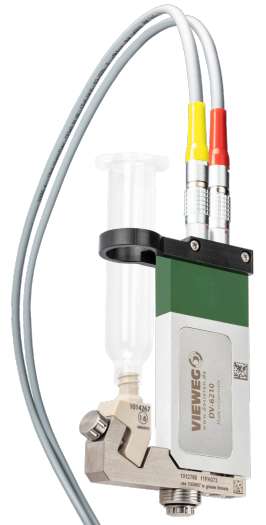
\includegraphics[width=0.25\linewidth]{Sections/6 Detaljeløsning/Media/Jetventil DV1.png}
    \caption{Billede af Jet valve DV-6210 fra: \parencite{VIEWEG2025JetDV-6210}.}
    \label{fig:Jetventil}
\end{figure}
\plainbreak{-0.5}

%Størrelsen af farvedråben på emnet, afhænger af farvemidlet, der benyttes til emnet, men dysehovedets åbning er udskiflig og kan købes med en diameter fra 0.03 mm til 1.2 mm. Det er derved blevet vurderet at Jet valve DV-6210 er et passende valg til produktet. 

Et komplet sæt Jet Valve DV-6210 fra VIEWEG inklusiv pumpe, kontrolsystem og dysehoveder koster €8.385 ($\approx 62.500 DKK$). Dens minimale vægt er \SI{260}{g}, uden farvemiddel. \parencite{VIEWEG2025JetDV-6210}. 


\renewcommand{\arraystretch}{1.3}
\begin{table}[H]
\setlength{\tabcolsep}{20pt}
 \centering
  \caption{Opsummering}
 \begin{tabular}{|c c|} \hline
 \multicolumn{2}{|c|}{\cellcolor{aaublue} \color{white} \textbf{VIEWEG DV-6210}}  \\\hline
 \rowcolor{gray!10} \multicolumn{1}{|c}{\textbf{Variabel}} &  \multicolumn{1}{c|}{\textbf{Værdi}}  \\\hline
 
 %PeJV &  VIEWEG DV-6210\\\hline
 Vægt &  $\geq \SI{260}{g} $\\\hline
 Minimal diameter på prikstørrelse &  $\diameter\SI{0,08}{mm}$\\\hline
 Prikker pr. sekund &  3000 \\\hline
 \end{tabular}
 \label{tab: PeJV opsummering}
\end{table}

%(skulle have stået mellem linje 19 go 21)%PeP blev fravalgt på baggrund af manlgede forsknings artikler og indrustri brug, af PeP dråbe dosering. Derudover blev PeJV valgt frem for TIJ, grundet den højere hastighed, der kan opereres med.